% =====================================================================
% Relatório - Prática 4: Ondas estacionárias
% Versão em arquivo único, no mesmo formato do Relatorio_Pratica3.tex;
% a única dependência externa é a imagem pags/imagens/usp-logo-0.png.
% =====================================================================
\documentclass[12pt, a4paper]{article}

% ======================== config/preambulo.tex ========================
\PassOptionsToPackage{table, dvipsnames}{xcolor}
\usepackage{xcolor}
\usepackage[utf8]{inputenc}
\usepackage[T1]{fontenc}
\usepackage[brazilian]{babel}

% ---------------------------------------------------------------
% Fonte, espaçamento e margens (ABNT NBR 14724)
% ---------------------------------------------------------------
\usepackage{mathptmx}
\usepackage{setspace}
\usepackage{indentfirst}
\onehalfspacing
\setlength{\parindent}{1.25cm}
\setlength{\emergencystretch}{2em}

\usepackage{geometry}
\geometry{
    a4paper,
    left=3cm,
    top=3cm,
    right=2cm,
    bottom=2cm
}

% ---------------------------------------------------------------
% Numeração de páginas no canto superior direito (ABNT NBR 14724)
% ---------------------------------------------------------------
\usepackage{fancyhdr}
\fancypagestyle{abnt}{%
    \fancyhf{}%
    \fancyhead[R]{\small\thepage}%
    \renewcommand{\headrulewidth}{0pt}%
}
\setlength{\headheight}{15pt}

% ---------------------------------------------------------------
% Matemática e unidades
% ---------------------------------------------------------------
\usepackage{amsmath}
\usepackage{amsfonts}
\usepackage{amssymb}
\usepackage{siunitx}
\sisetup{
    output-decimal-marker = {,},
    per-mode = symbol,
    separate-uncertainty = true
}
% unidade em texto reto, com espaço fino: $10\un{s}$
\newcommand{\un}[1]{\,\mathrm{#1}}
% citação numérica (ABNT NBR 10520, sistema numérico)
\newcommand{\cita}[1]{\textsuperscript{[#1]}}

% ---------------------------------------------------------------
% Figuras, tabelas e legendas (título acima, fonte abaixo)
% ---------------------------------------------------------------
\usepackage{graphicx}
\usepackage{float}
\usepackage{caption}
\captionsetup{
    labelsep = endash,
    justification = centering,
    font = {small, singlespacing},
    skip = 4pt
}
\usepackage{subcaption}
\usepackage{booktabs}
\usepackage{array}
\usepackage{multirow}
\newcommand{\fonte}[1]{\par\vspace{2pt}{\footnotesize Fonte: #1}}

\usepackage{pgfplots}
\pgfplotsset{
    compat = 1.17,
    every axis/.append style = {font=\small},
}
\pgfkeys{/pgf/number format/.cd, use comma, 1000 sep={}}

\usepackage[
    colorlinks=true,
    linkcolor=black,
    citecolor=black,
    urlcolor=black
]{hyperref}

\graphicspath{{./pags/imagens/}}



\begin{document}

% ======================== pags/0-Capa.tex ========================
\begin{titlepage}
    \centering
    \vspace*{-2cm}
    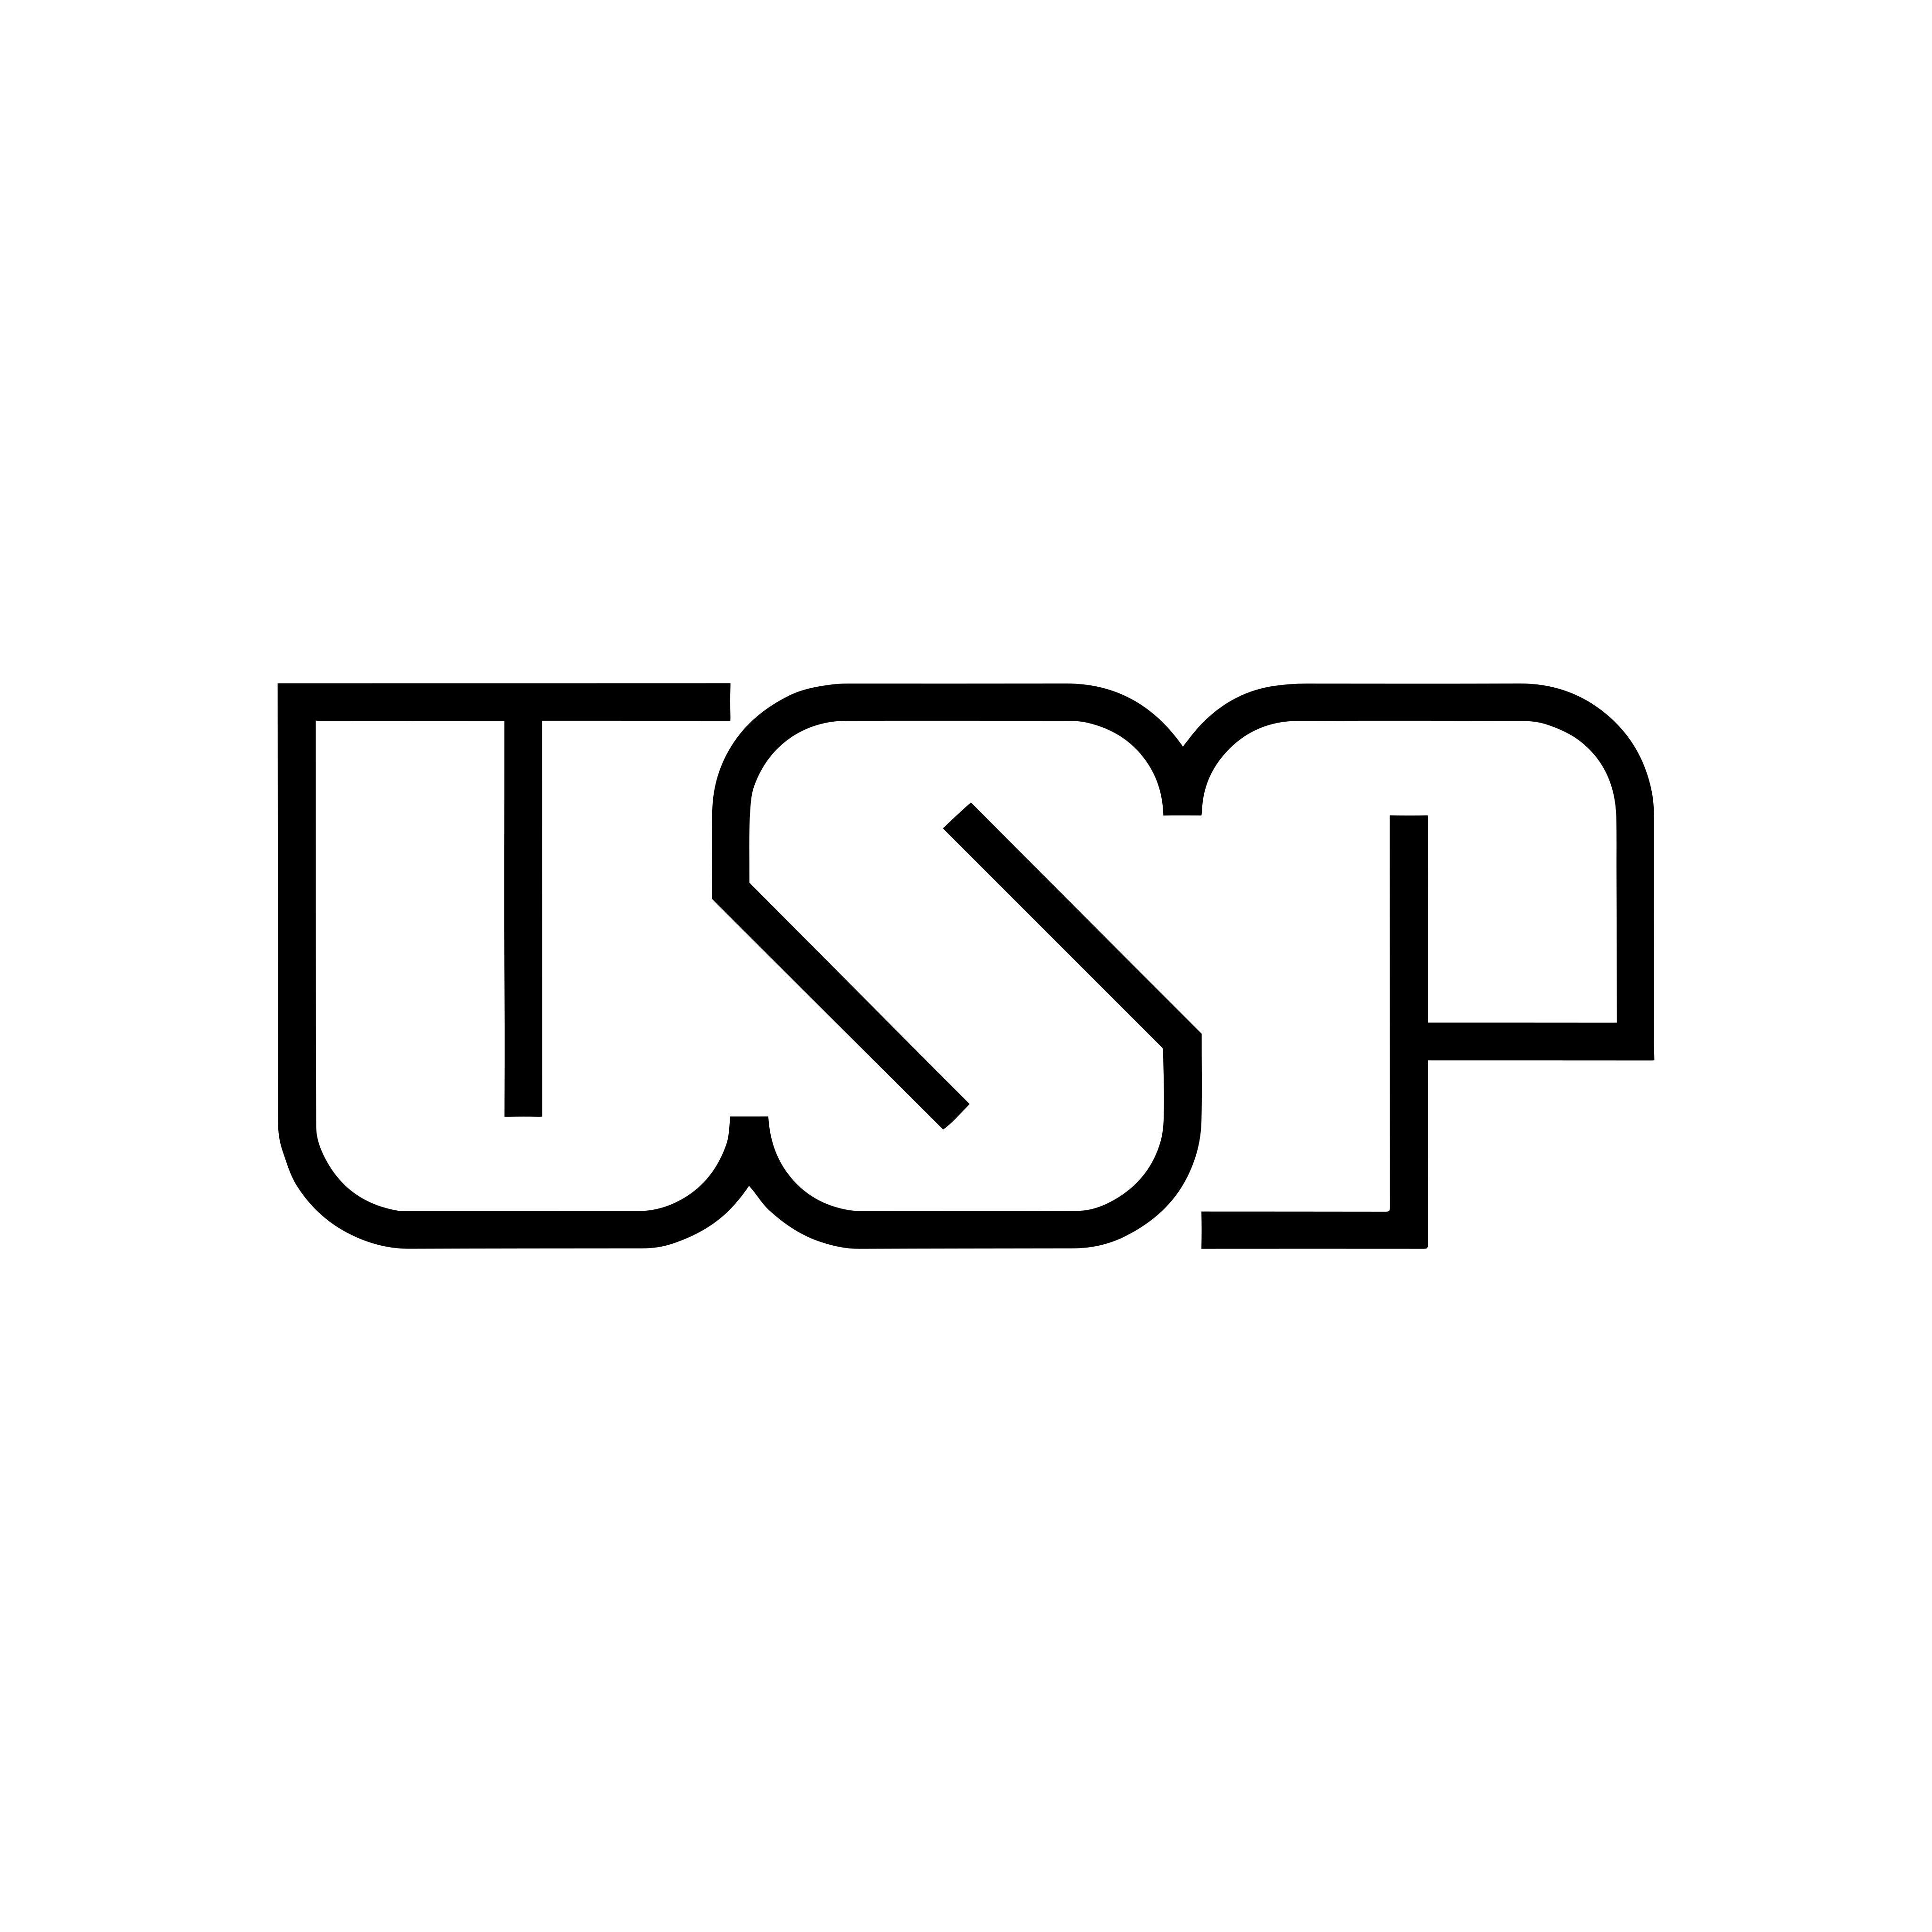
\includegraphics[width=10.0cm]{pags/imagens/usp-logo-0.png} \\[1.5cm]

    {\large \textbf{UNIVERSIDADE DE SÃO PAULO}} \\[0.3cm]
    {\large \textbf{DEPARTAMENTO DE ENGENHARIA MECÂNICA}} \\[0.3cm]
    {\large \textbf{LABORATÓRIO DE FÍSICA EXPERIMENTAL II}} \\[1cm]
    {\Large \textbf{Prática 4: Ondas estacionárias}} \\[0.4cm]
    {\large \textbf{PROFESSOR: Hai Guoqiang}} \\[1cm]
    {\large \textbf{INTEGRANTES:\\}
    Flávio Henrique Monteiro Silva - 17890005 \\
    Guilherme Tommasino Ribeiro - 17894232}
    \vfill
    {\large São Carlos-SP} \\[0.2cm]
    {\large \textbf{2026}}
\end{titlepage}
\clearpage


\setcounter{page}{2}
\thispagestyle{empty}
\tableofcontents
\clearpage

\pagestyle{abnt}
% ======================== pags/1-Introducao_e_Objetivos.tex ========================
\section{Introdução e Objetivos}

\subsection{Introdução}

Uma onda é uma perturbação que se propaga através de um meio, transportando energia sem que o meio acompanhe a propagação\cita{1}. Em uma corda tensionada, a perturbação é perpendicular à direção de propagação (onda transversal), e sua velocidade depende apenas das propriedades do meio: a tensão $F$ e a densidade linear de massa $\mu$, por meio de $v=\sqrt{F/\mu}$\cita{2}. Já o som é uma onda longitudinal de pressão, cuja velocidade no ar depende da temperatura e da pressão do gás\cita{3}.

Quando uma onda é refletida em uma extremidade e se superpõe à onda incidente, que viaja em sentido oposto com mesma amplitude e frequência, forma-se uma onda estacionária: um padrão de oscilação em que as cristas não se deslocam, com pontos de amplitude nula (nós) e de amplitude máxima (antinós) em posições fixas. Como as condições nas extremidades restringem os comprimentos de onda permitidos, somente certas frequências (os harmônicos) produzem ondas estacionárias em uma corda ou em uma coluna de ar de comprimento $L$\cita{1,2}. Medindo os comprimentos de onda e as frequências desses harmônicos, é possível determinar a velocidade de propagação das ondas progressivas em cada meio.

\subsection{Objetivos}

Este relatório tem como objetivo estudar o comportamento de ondas transversais estacionárias em cordas e de ondas sonoras estacionárias em colunas de ar, determinando a velocidade de propagação das ondas progressivas em cada um dos meios. Especificamente, busca-se:
\begin{itemize}
    \item gerar os harmônicos de uma corda com extremos fixos, determinar a velocidade da onda para cada harmônico, verificar se ela é constante e, a partir dela, calcular a densidade linear $\mu$ da corda, comparando-a com o valor obtido pela razão entre a massa e o comprimento de uma amostra da corda;
    \item gerar os harmônicos de uma coluna de ar de comprimento fixo variando a frequência, verificar a relação linear entre $f_n$ e $n$ e determinar a velocidade do som pelo método dos mínimos quadrados;
    \item gerar os harmônicos de uma coluna de ar com frequência fixa variando o comprimento, determinar o comprimento de onda e a velocidade do som e comparar com o resultado anterior e com o valor de referência;
    \item discutir as fontes de incerteza envolvidas em cada procedimento.
\end{itemize}

% ======================== pags/2-Materiais_e_Metodos.tex ========================
\section{Materiais e Métodos}

\subsection{Instrumentos e Materiais}

Para a realização do experimento, foram utilizados os seguintes instrumentos:
\begin{itemize}
    \item Gerador de funções (sinal senoidal) com mostrador digital de frequência;
    \item Vibrador formado por um alto-falante com um pino acoplado, no qual uma das extremidades da corda é presa;
    \item Corda, roldana e corpo de massa $m$ suspenso na outra extremidade da corda, que define a tensão aplicada;
    \item Amostra da mesma corda, de comprimento $(15{,}000\pm0{,}005)\un{m}$ e massa $(7{,}07\pm0{,}01)\un{g}$, para a determinação direta de $\mu$;
    \item Balança e trena;
    \item Tubo cilíndrico com alto-falante em uma das extremidades e, na outra, um pistão móvel acoplado a um microfone, com escala graduada em centímetros para a leitura do comprimento da coluna de ar;
    \item Osciloscópio, para a monitoração do sinal do microfone.
\end{itemize}

\subsection{Métodos}

Para uma melhor compreensão do procedimento experimental, além de melhorar a concepção cronológica das práticas, esta seção do relatório será dividida em três experimentos diferentes:
\begin{itemize}
    \item Ondas estacionárias na corda (experimento 1);
    \item Ondas estacionárias de som: harmônicos em função da frequência (experimento 2);
    \item Ondas estacionárias de som: harmônicos em função do comprimento (experimento 3).
\end{itemize}

\subsubsection{Experimento 1}

Uma das extremidades da corda foi presa ao pino do vibrador e a outra, após passar pela roldana, foi ligada ao corpo suspenso, mantendo-se constantes o comprimento vibrante $L$ e a tensão $F=mg$. O vibrador foi alimentado pelo gerador de funções, e a frequência foi aumentada lentamente a partir de valores baixos até o aparecimento de uma onda estacionária. Para cada harmônico $n$, identificado pela contagem dos ventres (antinós) ao longo da corda, a frequência foi ajustada cuidadosamente até a máxima amplitude de oscilação e registrada. Foram obtidos os seis primeiros harmônicos. O comprimento de onda de cada harmônico foi calculado pela condição de onda estacionária (Seção~\ref{sec:corda}), e a velocidade, por $v_n=\lambda_nf_n$. Com a velocidade média, determinou-se $\mu$, que foi comparada com o valor obtido pela razão entre a massa e o comprimento da amostra da corda.

\subsubsection{Experimento 2}

Com a bateria do microfone conectada e o gerador de funções ligado ao alto-falante, o pistão foi deslocado até que o comprimento da coluna de ar fosse $L=0{,}15\un{m}$. Partindo das menores frequências, para garantir a detecção do modo fundamental, a frequência do gerador foi aumentada até que o sinal do microfone no osciloscópio atingisse a máxima intensidade, condição que corresponde a uma onda estacionária no tubo. Registraram-se as frequências $f_n$ dos dez primeiros harmônicos sucessivos, que foram comparadas com os valores de referência calculados para $v=340\un{m/s}$. Com os dados, construiu-se o gráfico de $f_n$ em função de $n$ e determinou-se a velocidade do som pelo método dos mínimos quadrados.

\subsubsection{Experimento 3}

A frequência do gerador foi fixada próxima de $2\un{kHz}$, tendo sido lida no mostrador $f=2002{,}2\un{Hz}$. Começando com o pistão próximo ao alto-falante, para garantir a detecção do modo fundamental, o pistão foi afastado lentamente, e foram registrados os comprimentos $L_n$ da coluna de ar nos quais o sinal do microfone atingia intensidade máxima, correspondentes aos dez primeiros harmônicos. Com os dados, calcularam-se as diferenças entre comprimentos sucessivos, o comprimento de onda e a velocidade do som, posteriormente comparada com o resultado do Experimento 2.

\subsection{Dedução das Equações}

As deduções a seguir seguem a apostila da disciplina\cita{1} e as referências\cita{2,3}.

\subsubsection{Velocidade de uma onda transversal em uma corda}

Em uma corda de densidade linear $\mu$, tensionada por uma força $F$, uma perturbação transversal se propaga com velocidade
\begin{equation}
v=\sqrt{\frac{F}{\mu}}
\label{eq:vFmu}
\end{equation}
e, como uma crista percorre a distância $\lambda$ em um período $T=1/f$,
\begin{equation}
v=\frac{\lambda}{T}=\lambda f.
\label{eq:vlf}
\end{equation}
A velocidade depende apenas da tensão e da densidade da corda, e não da fonte que gera a onda. Como, no experimento, a tensão é o peso do corpo suspenso, $F=mg$, isolando $\mu$ na Equação~\eqref{eq:vFmu} obtém-se
\begin{equation}
\mu=\frac{F}{v^2}=\frac{mg}{v^2}.
\label{eq:mu}
\end{equation}

\subsubsection{Ondas estacionárias em uma corda com extremos fixos}
\label{sec:corda}

A onda gerada no vibrador e a onda refletida na extremidade oposta viajam em sentidos opostos com mesma amplitude e frequência. Como a equação de onda é linear, sua superposição também é solução:
\[
z(x,t)=A\cos(kx-\omega t)-A\cos(kx+\omega t)=2A\,\sin(kx)\,\sin(\omega t),
\]
em que o sinal negativo da onda refletida garante $z(0,t)=0$ para todo $t$ (extremo fixo em $x=0$). Essa é uma onda estacionária: cada ponto da corda oscila com frequência $f$ e amplitude $2A|\sin(kx)|$, que não se desloca ao longo da corda. Impondo que o outro extremo, $x=L$, também seja fixo, $z(L,t)=0$, isto é, $\sin(kL)=0$, de onde $kL=n\pi$, com $n=1,2,3,\dots$ Como $k=2\pi/\lambda$, os comprimentos de onda permitidos são
\begin{equation}
L=n\,\frac{\lambda_n}{2}
\quad\Longrightarrow\quad
\lambda_n=\frac{2L}{n},
\label{eq:ln}
\end{equation}
em que $n$ é o índice do harmônico. Os nós ocorrem em $x=j\lambda_n/2$ ($j=0,1,\dots,n$), totalizando $n+1$ nós (incluindo as extremidades) e $n$ antinós. Como a velocidade é a mesma para todos os harmônicos, a Equação~\eqref{eq:vlf} fornece
\begin{equation}
f_n=\frac{v}{\lambda_n}=n\,\frac{v}{2L}=n\,f_1,
\label{eq:fn}
\end{equation}
isto é, as frequências dos harmônicos são múltiplos inteiros da frequência fundamental $f_1=v/2L$.

\subsubsection{Ondas sonoras estacionárias em um tubo fechado}

No tubo, a onda sonora emitida pelo alto-falante é refletida no pistão e superpõe-se à onda incidente. Em uma parede rígida, o deslocamento das moléculas de ar é nulo e a pressão apresenta um antinó (crista); o mesmo ocorre, aproximadamente, junto à membrana do alto-falante\cita{1}. Como há um antinó de pressão em cada extremidade e antinós consecutivos estão separados por meio comprimento de onda (Figura 4.2 da apostila\cita{1}), o comprimento do tubo deve ser um múltiplo inteiro de $\lambda/2$. Obtém-se, portanto, a mesma condição da corda:
\begin{equation}
L=n\,\frac{\lambda_n}{2},
\qquad
f_n=n\,\frac{v}{2L}.
\label{eq:fsom}
\end{equation}
Para um tubo de comprimento $L$ fixo, as frequências dos harmônicos são proporcionais a $n$, e o gráfico de $f_n$ em função de $n$ deve ser uma reta que passa pela origem, com coeficiente angular
\begin{equation}
b=\frac{v}{2L}
\quad\Longrightarrow\quad
v=2Lb.
\label{eq:v2Lb}
\end{equation}

Se, por outro lado, a frequência $f$ for fixa, o comprimento de onda $\lambda=v/f$ é constante, e as ondas estacionárias ocorrem para os comprimentos de coluna
\begin{equation}
L_n=n\,\frac{\lambda}{2},
\qquad
\lambda_n=\frac{2L_n}{n},
\label{eq:Ln}
\end{equation}
de modo que a diferença entre comprimentos sucessivos deve ser constante e igual a meio comprimento de onda, $L_{n+1}-L_n=\lambda/2$. Conhecido $\lambda$, a velocidade do som é $v=\lambda f$.

Neste relatório, adota-se como valor de referência para a velocidade do som no ar $v_{ref}=340\un{m/s}$, conforme indicado no roteiro.

% ======================== pags/3-Resultados_experimentais.tex ========================
\section{Resultados e Discussões}

Conforme orientação do roteiro, as grandezas obtidas a partir de vários harmônicos foram expressas pela média, com incerteza dada pelo desvio médio, isto é, a média dos módulos das diferenças entre cada valor e a média. Os coeficientes das retas e suas incertezas foram obtidos pelo método dos mínimos quadrados (MMQ). Os resultados foram arredondados apenas ao final dos cálculos.

\subsection{Ondas estacionárias na corda}

\subsubsection{Velocidade da onda}

O comprimento vibrante da corda foi $L=1{,}0\un{m}$, e a massa suspensa, $m=182{,}77\un{g}$. Para cada harmônico, o comprimento de onda foi calculado pela Equação~\eqref{eq:ln}, $\lambda_n=2L/n$, e a velocidade, pela Equação~\eqref{eq:vlf}, $v_n=\lambda_nf_n$. Por exemplo, para $n=3$,
\begin{gather*}
\lambda_3=\frac{2\cdot1{,}0}{3}=0{,}667\un{m},\\
v_3=0{,}667\cdot550=366{,}7\un{m/s}.
\end{gather*}
A média das seis velocidades é
\[
\bar{v}=\frac{340{,}0+350{,}0+366{,}7+355{,}0+360{,}0+360{,}0}{6}=355{,}28\un{m/s},
\]
e os desvios $|v_n-\bar{v}|$ correspondentes estão na Tabela~\ref{tab:corda}, que reúne os dados e os resultados.

\begin{table}[H]
\centering
\caption{Harmônicos da corda com $L=1{,}0\un{m}$ e $m=182{,}77\un{g}$.}
\label{tab:corda}
\begin{tabular}{ccccc}
\toprule
$n$ & $\lambda_n$ (m) & $f_n$ (Hz) & $v_n$ (m/s) & $|v_n-\bar{v}|$ (m/s) \\
\midrule
1 & 2,000 & 170 & 340,0 & 15,3 \\
2 & 1,000 & 350 & 350,0 & 5,3 \\
3 & 0,667 & 550 & 366,7 & 11,4 \\
4 & 0,500 & 710 & 355,0 & 0,3 \\
5 & 0,400 & 900 & 360,0 & 4,7 \\
6 & 0,333 & 1080 & 360,0 & 4,7 \\
\bottomrule
\end{tabular}
\fonte{Elaborada pelos autores.}
\end{table}

O desvio médio é
\[
\Delta v=\frac{15{,}28+5{,}28+11{,}39+0{,}28+4{,}72+4{,}72}{6}=6{,}94\un{m/s},
\]
de modo que a velocidade da onda na corda é
\[
v=(355\pm7)\un{m/s}.
\]
A Figura~\ref{fig:vn} mostra as velocidades obtidas para cada harmônico. Todos os valores diferem da média em no máximo $4{,}3\%$, e não há tendência sistemática com $n$; dentro da dispersão experimental, a velocidade pode ser considerada constante, como previsto, já que ela depende apenas da tensão e da densidade da corda (Equação~\ref{eq:vFmu}), que não foram alteradas. A maior diferença ocorre para $n=1$, harmônico em que a frequência é a menor e o ajuste da máxima amplitude é mais difícil, e para $n=3$. Como as frequências foram anotadas com resolução de $10\un{Hz}$, uma incerteza de leitura de $\pm5\un{Hz}$ corresponde a $\pm3\%$ em $f_1$, comparável à dispersão observada.

\begin{figure}[H]
\centering
\caption{Velocidade $v_n=\lambda_nf_n$ em função do índice do harmônico para a corda.}
\label{fig:vn}
\begin{tikzpicture}
\begin{axis}[
  width=0.82\textwidth, height=6.5cm,
  xlabel={$n$}, ylabel={$v_n$ (m/s)},
  xmin=0.5, xmax=6.5, ymin=320, ymax=385,
  xtick={1,2,3,4,5,6},
  grid=both, legend pos=south east, legend style={font=\footnotesize},
]
\addplot[only marks, mark=*, mark size=2pt] coordinates {
(1,340) (2,350) (3,366.667) (4,355) (5,360) (6,360)
};
\addlegendentry{dados}
\addplot[thick, domain=0.5:6.5] {355.28};
\addlegendentry{$\bar{v}=355{,}3\un{m/s}$}
\addplot[dashed, domain=0.5:6.5, forget plot] {355.28+6.94};
\addplot[dashed, domain=0.5:6.5] {355.28-6.94};
\addlegendentry{$\bar{v}\pm\Delta v$}
\end{axis}
\end{tikzpicture}
\fonte{Elaborada pelos autores.}
\end{figure}

\subsubsection{Densidade linear da corda}

A tensão na corda é o peso do corpo suspenso,
\[
F=mg=\left(182{,}77\times10^{-3}\right)(9{,}81)=1{,}7930\un{N}.
\]
Com a velocidade medida, a Equação~\eqref{eq:mu} fornece
\begin{gather*}
\mu=\frac{F}{\bar{v}^2}=\frac{1{,}7930}{(355{,}28)^2}=1{,}420\times10^{-5}\un{kg/m},\\
\frac{u(\mu)}{\mu}=\sqrt{\left(\frac{0{,}01}{182{,}77}\right)^2+\left(\frac{2\cdot6{,}94}{355{,}28}\right)^2}=0{,}039,
\end{gather*}
isto é, $\mu=(1{,}42\pm0{,}06)\times10^{-5}\un{kg/m}=(0{,}0142\pm0{,}0006)\un{g/m}$. A incerteza da massa (resolução da balança, $0{,}01\un{g}$) é desprezível frente à da velocidade.

A densidade linear da corda utilizada, obtida pela massa e pelo comprimento da amostra, é
\begin{gather*}
\mu_{real}=\frac{m_c}{L_c}=\frac{7{,}07}{15{,}000}=0{,}4713\un{g/m},\\
\frac{u(\mu_{real})}{\mu_{real}}=\sqrt{\left(\frac{0{,}01}{7{,}07}\right)^2+\left(\frac{0{,}005}{15{,}000}\right)^2}=0{,}0015,
\end{gather*}
ou seja, $\mu_{real}=(0{,}4713\pm0{,}0007)\un{g/m}=(4{,}713\pm0{,}007)\times10^{-4}\un{kg/m}$.

O valor obtido a partir da velocidade da onda é menor que o valor nominal da corda. Para interpretar essa diferença, é útil comparar as velocidades. Com $\mu_{real}$ e a tensão aplicada, a Equação~\eqref{eq:vFmu} fornece
\begin{gather*}
v_{nom}=\sqrt{\frac{F}{\mu_{real}}}=\sqrt{\frac{1{,}7930}{4{,}713\times10^{-4}}}=61{,}7\un{m/s},
\end{gather*}
enquanto a velocidade obtida dos harmônicos foi de $355\un{m/s}$. Como $\mu$ depende do inverso do quadrado da velocidade, a diferença entre as velocidades aparece ampliada em $\mu$.

As frequências medidas apresentam a proporção $f_n\approx n\,f_1$ esperada para harmônicos (a regressão linear de $f_n$ em função de $n$ fornece coeficiente angular de $181{,}7\un{Hz}$ e coeficiente linear de $-9{,}3\un{Hz}$, próximo de zero), o que confirma a formação das ondas estacionárias e a relação $f_n=n\,v/2L$. A diferença entre os valores de $\mu$ pode ser associada a fatores da montagem que não são contemplados pelo modelo ideal:
\begin{enumerate}
    \item o comprimento que efetivamente vibra é delimitado pelo pino do vibrador e pelo ponto de contato da corda com a roldana, e o valor de $v$ obtido é diretamente proporcional ao comprimento adotado ($v_n=2Lf_n/n$);
    \item o vibrador excita com mais eficiência alguns modos do que outros, de modo que a identificação do índice $n$ de cada padrão observado depende da contagem visual dos ventres;
    \item o próprio vibrador (alto-falante) possui ressonâncias mecânicas, que reforçam a amplitude em determinadas faixas de frequência;
    \item o modelo considera a corda perfeitamente flexível e de extremos rigidamente fixos, enquanto o pino oscila e a roldana apresenta atrito e inércia, o que altera a tensão efetiva ao longo da corda.
\end{enumerate}

\subsection{Ondas sonoras estacionárias: harmônicos em função da frequência}

Para o tubo com $L=0{,}15\un{m}$ e $v_{ref}=340\un{m/s}$, a Equação~\eqref{eq:fsom} prevê
\[
f_1^{ref}=\frac{v_{ref}}{2L}=\frac{340}{2\cdot0{,}15}=1133{,}3\un{Hz},
\qquad
f_n^{ref}=n\cdot1133{,}3\un{Hz}.
\]
A Tabela~\ref{tab:som_f} apresenta as frequências medidas e os valores de referência.

\begin{table}[H]
\centering
\caption{Frequências dos harmônicos no tubo com $L=0{,}15\un{m}$.}
\label{tab:som_f}
\begin{tabular}{cccc}
\toprule
$n$ & $f_n^{ref}$ (Hz) & $f_n$ (Hz) & $(f_n-f_n^{ref})/f_n^{ref}$ (\%) \\
\midrule
1 & 1133 & 1131 & $-0{,}2$ \\
2 & 2267 & 2247 & $-0{,}9$ \\
3 & 3400 & 3160 & $-7{,}1$ \\
4 & 4533 & 4210 & $-7{,}1$ \\
5 & 5667 & 5376 & $-5{,}1$ \\
6 & 6800 & 6388 & $-6{,}1$ \\
7 & 7933 & 7485 & $-5{,}7$ \\
8 & 9067 & 8547 & $-5{,}7$ \\
9 & 10200 & 9885 & $-3{,}1$ \\
10 & 11333 & 10732 & $-5{,}3$ \\
\bottomrule
\end{tabular}
\fonte{Elaborada pelos autores.}
\end{table}

A Figura~\ref{fig:som_f} mostra o gráfico de $f_n$ em função de $n$. Os pontos se alinham em uma reta que passa aproximadamente pela origem, isto é, observa-se uma relação de proporcionalidade direta entre $f_n$ e $n$, coerente com a Equação~\eqref{eq:fsom}, que define as ondas estacionárias no tubo fechado.

\begin{figure}[H]
\centering
\caption{Frequência dos harmônicos em função de $n$ para o tubo com $L=0{,}15\un{m}$.}
\label{fig:som_f}
\begin{tikzpicture}
\begin{axis}[
  width=0.85\textwidth, height=7.5cm,
  xlabel={$n$}, ylabel={$f_n$ (Hz)},
  xmin=0, xmax=11, ymin=0, ymax=12500,
  xtick={0,1,...,10},
  scaled y ticks=false,
  grid=both, legend pos=north west, legend style={font=\footnotesize},
]
\addplot[only marks, mark=*, mark size=2pt] coordinates {
(1,1131) (2,2247) (3,3160) (4,4210) (5,5376) (6,6388) (7,7485) (8,8547) (9,9885) (10,10732)
};
\addlegendentry{dados}
\addplot[thick, domain=0:11] {-5.47+1076.65*x};
\addlegendentry{ajuste: $f_n=-5{,}5+1076{,}6\,n$}
\addplot[dashed, domain=0:11] {1133.33*x};
\addlegendentry{referência ($v=340\un{m/s}$)}
\end{axis}
\end{tikzpicture}
\fonte{Elaborada pelos autores.}
\end{figure}

Aplicando o método dos mínimos quadrados aos dez pontos $(n,f_n)$, obteve-se
\begin{gather*}
b=(1076{,}6\pm10{,}8)\un{Hz},\\
a=(-5\pm67)\un{Hz},\\
r=0{,}9996.
\end{gather*}
Pela Equação~\eqref{eq:v2Lb}, a velocidade do som é
\begin{gather*}
v=2Lb=2\cdot0{,}15\cdot1076{,}6=323{,}0\un{m/s},\\
u(v)=2\cdot0{,}15\cdot10{,}8=3{,}2\un{m/s},
\end{gather*}
isto é,
\[
v=(323\pm3)\un{m/s}.
\]
O valor é $5{,}0\%$ menor que o de referência ($340\un{m/s}$), diferença de cerca de cinco vezes a incerteza, e, portanto, significativa.

O coeficiente linear deveria ser nulo, pois, pela Equação~\eqref{eq:fsom}, $f_n=n\,v/2L$ não possui termo independente (para $n=0$ não há onda). O valor obtido, $a=(-5\pm67)\un{Hz}$, é compatível com zero, de modo que o resultado é coerente com o modelo; a incerteza de $a$ é grande porque os pontos estão distantes da origem ($\bar{n}=5{,}5$).

Para garantir que o primeiro harmônico observado corresponde a $n=1$, o experimento foi iniciado nas menores frequências, aumentando-as gradualmente, e não foi observada nenhuma ressonância abaixo de $1131\un{Hz}$. Além disso, a razão entre as duas primeiras frequências é $2247/1131=1{,}99\approx2$; caso o primeiro máximo correspondesse a $n=2$, as frequências guardariam a razão $3/2$, e deveria haver uma ressonância em torno de $566\un{Hz}$. A frequência esperada para o modo fundamental no tubo utilizado é $f_1^{ref}=1133\un{Hz}$, que coincide com a menor frequência da tabela, $1131\un{Hz}$ (diferença de $0{,}2\%$), confirmando que ela corresponde ao modo fundamental.

A Tabela~\ref{tab:som_f} mostra que os dois primeiros harmônicos concordam com a referência, mas, a partir de $n=3$, as frequências medidas ficam sistematicamente entre $3\%$ e $7\%$ abaixo dela. Como o desvio é aproximadamente proporcional a $n$, ele corresponde a uma redução do coeficiente angular. Algumas causas plausíveis são:
\begin{enumerate}
    \item a crista de pressão junto ao alto-falante não se localiza exatamente na abertura do tubo\cita{4}, de modo que o comprimento efetivo da coluna de ar, $L+\delta$, é um pouco maior que o lido na escala. O coeficiente angular obtido corresponde a um comprimento efetivo $L_{ef}=v_{ref}/2b=340/(2\cdot1076{,}6)=0{,}158\un{m}$, ou seja, $\delta\approx0{,}8\un{cm}$, valor muito próximo da correção obtida de forma independente no Experimento 3 ($\delta=0{,}75\un{cm}$, Seção~\ref{sec:som_L}). Utilizando esse valor, $v=2(L+\delta)b=2\cdot0{,}1575\cdot1076{,}6=339\un{m/s}$, em ótima concordância com a referência;
    \item o comprimento $L=0{,}15\un{m}$ foi ajustado de forma aproximada na escala do tubo, e sua incerteza não foi incluída em $u(v)$; uma diferença de $0{,}5\un{cm}$ em $L$ altera $v$ em $3\%$;
    \item em altas frequências, a resposta do alto-falante e do microfone varia com a frequência e os picos de ressonância se tornam menos nítidos no osciloscópio.
\end{enumerate}

\subsection{Ondas sonoras estacionárias: harmônicos em função do comprimento}
\label{sec:som_L}

Com a frequência fixa em $f=2002{,}2\un{Hz}$, o comprimento de onda de referência é $\lambda_{ref}=v_{ref}/f=34000/2002{,}2=16{,}98\un{cm}$, e os comprimentos de ressonância esperados, pela Equação~\eqref{eq:Ln}, são $L_n^{ref}=n\cdot8{,}49\un{cm}$. A Tabela~\ref{tab:som_L} apresenta os comprimentos medidos, as diferenças entre valores sucessivos, os comprimentos de onda $\lambda_n=2L_n/n$ e os desvios em relação à média.

\begin{table}[H]
\centering
\caption{Comprimentos de ressonância da coluna de ar para $f=2002{,}2\un{Hz}$.}
\label{tab:som_L}
\begin{tabular}{cccccc}
\toprule
$n$ & $L_n^{ref}$ (cm) & $L_n$ (cm) & $L_{n+1}-L_n$ (cm) & $\lambda_n$ (cm) & $|\lambda_n-\bar{\lambda}|$ (cm) \\
\midrule
1 & 8,49 & 8,0 & 8,4 & 16,00 & 0,81 \\
2 & 16,98 & 16,4 & 8,6 & 16,40 & 0,41 \\
3 & 25,47 & 25,0 & 8,8 & 16,67 & 0,15 \\
4 & 33,96 & 33,8 & 8,6 & 16,90 & 0,09 \\
5 & 42,45 & 42,4 & 8,6 & 16,96 & 0,15 \\
6 & 50,94 & 51,0 & 8,5 & 17,00 & 0,19 \\
7 & 59,43 & 59,5 & 8,5 & 17,00 & 0,19 \\
8 & 67,93 & 68,0 & 9,0 & 17,00 & 0,19 \\
9 & 76,42 & 77,0 & 8,5 & 17,11 & 0,30 \\
10 & 84,91 & 85,5 & --- & 17,10 & 0,29 \\
\bottomrule
\end{tabular}
\fonte{Elaborada pelos autores.}
\end{table}

De acordo com a Equação~\eqref{eq:Ln}, as diferenças entre comprimentos sucessivos deveriam ser constantes e iguais a $\lambda/2$. De fato, elas variam apenas entre $8{,}4$ e $9{,}0\un{cm}$, com média $8{,}61\un{cm}$ e desvio médio $0{,}13\un{cm}$, compatível com a resolução de leitura da posição do pistão. Esse resultado corresponde a $\lambda=2\cdot8{,}61=(17{,}2\pm0{,}3)\un{cm}$.

\subsubsection{Comprimento de onda e velocidade pela média}

Seguindo o procedimento do roteiro, a média dos dez comprimentos de onda $\lambda_n=2L_n/n$ da Tabela~\ref{tab:som_L} e seu desvio médio são
\begin{gather*}
\bar{\lambda}=\frac{16{,}00+16{,}40+16{,}67+16{,}90+16{,}96+3\cdot17{,}00+17{,}11+17{,}10}{10}=16{,}81\un{cm},\\
\Delta\lambda=\frac{0{,}81+0{,}41+0{,}15+0{,}09+0{,}15+0{,}19+0{,}19+0{,}19+0{,}30+0{,}29}{10}=0{,}27\un{cm},
\end{gather*}
isto é, $\lambda=(16{,}8\pm0{,}3)\un{cm}$. A velocidade do som resulta em
\begin{gather*}
v=\bar{\lambda}f=0{,}16814\cdot2002{,}2=336{,}6\un{m/s},\\
\Delta v=f\,\Delta\lambda=2002{,}2\cdot0{,}00275=5{,}5\un{m/s},
\end{gather*}
ou seja,
\[
v=(337\pm6)\un{m/s},
\]
compatível com o valor de referência de $340\un{m/s}$ (diferença de $1{,}0\%$, menor que a incerteza).

Observa-se, entretanto, na Tabela~\ref{tab:som_L}, que $\lambda_n$ cresce sistematicamente com $n$, de $16{,}00\un{cm}$ para $n=1$ até aproximadamente $17{,}1\un{cm}$ para $n\ge9$. Esse comportamento é explicado pela diferença $\delta$ entre o comprimento efetivo da coluna e o lido na escala: se cada $L_n$ medido é menor que o efetivo por um mesmo valor $\delta$, então $\lambda_n=2L_n/n$ fica menor que $\lambda$ por $2\delta/n$, diferença que é maior para os primeiros harmônicos e diminui com $n$. Assim, a média simples de $\lambda_n$ é deslocada para valores menores, e o desvio médio reflete principalmente esse efeito sistemático, e não a dispersão aleatória.

\subsubsection{Comprimento de onda e velocidade pelo método dos mínimos quadrados}

Para eliminar esse efeito, ajustou-se a reta $L_n=a+b\,n$ aos dez pontos. Pela Equação~\eqref{eq:Ln}, o coeficiente angular é $b=\lambda/2$, e a diferença constante $\delta$ aparece apenas no coeficiente linear, $a=-\delta$, sem afetar $b$. A Figura~\ref{fig:som_L} mostra os dados e a reta ajustada.

\begin{figure}[H]
\centering
\caption{Comprimento de ressonância da coluna de ar em função de $n$ para $f=2002{,}2\un{Hz}$.}
\label{fig:som_L}
\begin{tikzpicture}
\begin{axis}[
  width=0.85\textwidth, height=7.5cm,
  xlabel={$n$}, ylabel={$L_n$ (cm)},
  xmin=0, xmax=11, ymin=-2, ymax=95,
  xtick={0,1,...,10},
  grid=both, legend pos=north west, legend style={font=\footnotesize},
]
\addplot[only marks, mark=*, mark size=2pt] coordinates {
(1,8.0) (2,16.4) (3,25.0) (4,33.8) (5,42.4) (6,51.0) (7,59.5) (8,68.0) (9,77.0) (10,85.5)
};
\addlegendentry{dados}
\addplot[thick, domain=0:11] {-0.753+8.6206*x};
\addlegendentry{ajuste: $L_n=-0{,}75+8{,}621\,n$}
\addplot[dashed, domain=0:11] {8.4907*x};
\addlegendentry{referência ($v=340\un{m/s}$)}
\end{axis}
\end{tikzpicture}
\fonte{Elaborada pelos autores.}
\end{figure}

Pelo método dos mínimos quadrados, obteve-se
\begin{gather*}
b=(8{,}621\pm0{,}014)\un{cm},\\
a=(-0{,}75\pm0{,}09)\un{cm},\\
r=0{,}99999.
\end{gather*}
O coeficiente de correlação muito próximo de 1 confirma a relação linear prevista. O comprimento de onda e a velocidade do som resultam em
\begin{gather*}
\lambda=2b=17{,}24\un{cm},\qquad u(\lambda)=2\,u(b)=0{,}028\un{cm},\\
v=\lambda f=0{,}17241\cdot2002{,}2=345{,}2\un{m/s},\qquad u(v)=2002{,}2\cdot0{,}00028=0{,}6\un{m/s},
\end{gather*}
ou seja, $\lambda=(17{,}24\pm0{,}03)\un{cm}$ e
\[
v=(345{,}2\pm0{,}6)\un{m/s}.
\]
O valor difere em $1{,}5\%$ do de referência. O coeficiente linear, $a=(-0{,}75\pm0{,}09)\un{cm}$, é significativamente diferente de zero e corresponde a $\delta=(0{,}75\pm0{,}09)\un{cm}$, isto é, o comprimento efetivo da coluna de ar é $0{,}75\un{cm}$ maior que o lido na escala, possivelmente porque a crista de pressão junto ao alto-falante não se localiza exatamente na abertura do tubo\cita{4}.

\subsubsection{Comparação entre os Experimentos 2 e 3}

A Tabela~\ref{tab:comparacao} resume os valores da velocidade do som obtidos.

\begin{table}[H]
\centering
\caption{Velocidade do som obtida por cada método.}
\label{tab:comparacao}
\begin{tabular}{lc}
\toprule
Método & $v$ (m/s) \\
\midrule
$f_n$ vs.\ $n$ com $L=0{,}15\un{m}$ (MMQ) & $323\pm3$ \\
$f_n$ vs.\ $n$ com $L+\delta=0{,}1575\un{m}$ & $339\pm3$ \\
Média de $\lambda_n=2L_n/n$ & $337\pm6$ \\
Diferenças $L_{n+1}-L_n$ & $345\pm5$ \\
$L_n$ vs.\ $n$ (MMQ) & $345{,}2\pm0{,}6$ \\
\midrule
Referência do roteiro & 340 \\
\bottomrule
\end{tabular}
\fonte{Elaborada pelos autores.}
\end{table}

O valor do Experimento 2, $(323\pm3)\un{m/s}$, é menor que o do Experimento 3 e não é compatível com ele. Os dois experimentos, contudo, estão sujeitos à mesma correção de extremidade, que afeta de modos diferentes cada método: no Experimento 2, ela entra diretamente em $v=2Lb$ e reduz o resultado em cerca de $5\%$, pois $\delta/L=0{,}75/15=5\%$; no Experimento 3, ela é absorvida pelo coeficiente linear da reta e não afeta o coeficiente angular. Corrigindo o comprimento do tubo pelo $\delta$ obtido no Experimento 3, o resultado do Experimento 2 passa a $(339\pm3)\un{m/s}$, próximo do valor de referência e a cerca de $2\%$ do obtido no Experimento 3. Conclui-se que o método do Experimento 3 (frequência fixa e comprimento variável, com ajuste linear) é o mais preciso, já que utiliza apenas diferenças de posição e não depende do conhecimento exato da posição da crista de pressão junto ao alto-falante.

% ======================== pags/4-Conclusao.tex ========================
\section{Conclusão}

Os experimentos permitiram observar ondas estacionárias em uma corda com extremos fixos e em uma coluna de ar em um tubo fechado, confirmando que, em ambos os casos, os harmônicos satisfazem a condição $L=n\lambda_n/2$.

Na corda, as frequências dos seis primeiros harmônicos foram aproximadamente múltiplos inteiros da fundamental, e a velocidade da onda foi praticamente constante entre os harmônicos, com $v=(355\pm7)\un{m/s}$. A densidade linear obtida a partir dessa velocidade e da tensão aplicada foi $\mu=(1{,}42\pm0{,}06)\times10^{-5}\un{kg/m}$, menor que o valor nominal da corda, $\mu_{real}=(4{,}713\pm0{,}007)\times10^{-4}\un{kg/m}$, diferença associada a características da montagem não contempladas pelo modelo ideal, como o comprimento efetivo de vibração e a resposta do vibrador.

No tubo com $L=0{,}15\un{m}$, a frequência fundamental medida, $1131\un{Hz}$, coincidiu com a esperada ($1133\un{Hz}$), e o gráfico de $f_n$ em função de $n$ mostrou relação linear, com coeficiente linear compatível com zero. A velocidade do som obtida pelo coeficiente angular, $(323\pm3)\un{m/s}$, ficou $5\%$ abaixo da referência, desvio explicado pela correção de extremidade do tubo. Com frequência fixa de $2002{,}2\un{Hz}$, as diferenças entre comprimentos de ressonância sucessivos foram praticamente constantes, como previsto, e o ajuste linear de $L_n$ em função de $n$ forneceu $\lambda=(17{,}24\pm0{,}03)\un{cm}$, $v=(345{,}2\pm0{,}6)\un{m/s}$ e uma correção de extremidade $\delta=(0{,}75\pm0{,}09)\un{cm}$. Aplicando essa correção ao Experimento 2, obteve-se $v=(339\pm3)\un{m/s}$, o que torna os dois experimentos coerentes entre si e com o valor de referência.

Assim, a prática permitiu compreender experimentalmente a formação de ondas estacionárias e a determinação da velocidade de propagação de ondas em diferentes meios, além de evidenciar a importância de considerar efeitos como a correção de extremidade na análise dos resultados.

% ======================== pags/5-Bibliografia.tex ========================
\section{Bibliografia}

\begin{enumerate}
    \item SCHNEIDER, J. F.; AZEVEDO, E. R. (comp.). \textbf{Laboratório de Física II}: livro de práticas. São Carlos: Instituto de Física de São Carlos, 2018.
    \item HALLIDAY, D.; RESNICK, R.; WALKER, J. \textbf{Fundamentos de física}: gravitação, ondas e termodinâmica. 10. ed. Rio de Janeiro: LTC, 2016. v. 2.
    \item NUSSENZVEIG, H. M. \textbf{Curso de física básica}: fluidos, oscilações e ondas, calor. 5. ed. São Paulo: Blucher, 2014. v. 2.
    \item PIZETTA, D. C.; WANDERLEY, A. B.; MASTELARO, V. R.; PAIVA, F. F. Uma avaliação experimental do tubo de ondas sonoras estacionárias. \textbf{Revista Brasileira de Ensino de Física}, São Paulo, v. 39, n. 3, e3301, 2017.
\end{enumerate}


\end{document}
